\section{Streams}\label{sec:streams}

\subsection{Streams and stream operators}\label{sec:notation}

$\N$ is the set of natural numbers, $\B$ is the set of Booleans, and $\Z$ is the set of integers.
$[n] = \{ 0, 1, 2, \ldots n-1 \}$ is the set of natural numbers less than n.

\begin{definition}[stream]
Given a set $A$, a \defined{stream} \emph{of values from $A$}, or an \emph{$A$-stream}, is a function $\N \rightarrow A$.
We denote by $\stream{A} \defn \{ s \,|\, s : \N \to A \}$ the set of all $A$-streams.
\end{definition}

When $s\in\stream{A}$ and $t\in\N$ we
write $s[t]$ for the $t$-th element of the stream $s$ instead of the usual $s(t)$
to distinguish it from other function applications.

We usually think of the index $t\in\N$ as (discrete) time and of $s[t]\in A$
as the value of the the stream $s$ ``at time'' $t$.

For example, the stream of natural numbers given by $\id[t] = t$ is the sequence of values
$\sv{0 1 2 3 4}$.

\begin{comment}
\begin{definition}
A \defined{finite stream} with $n$ values from $A$ is a function $[n] \to A$.
\end{definition}

A prefix of a stream is a finite stream.  For example, the prefix of $\id$ containing
the first 5 values is the finite stream
$[\begin{array}{ccccc} 0 & 1 & 2 & 3 & 4 \end{array}]$.
\end{comment}

\begin{definition}[stream operator]
A (typed) \defined{stream operator} with $n$ inputs is a function $T:\stream{A_0}\times\cdots\times\stream{A_{n-1}}\to\stream{B}$.
\end{definition}

In general we will use ``operator'' for functions on streams, and
``function'' for computations on ``scalar'' values.

\dbsp is an extension of the simply-typed lambda calculus -- we
introduce its elements gradually.  However, we find it more readable
to also use signal-processing-like circuit diagrams to depict \dbsp
programs.

Stream operator \emph{composition} (function composition) is shown as chained circuits.
The composition of a binary operator $T: \stream{A} \times \stream{B} \to \stream{A}$ with the
unary operator $S: \stream{A} \to \stream{B}$ into the computation
$\lambda s. T(T(s,S(s)),S(s)) : \stream{A}\to\stream{A}$
is given by the following circuit:

\begin{center}
\begin{tikzpicture}[auto,>=latex,minimum width=.5cm]
  \node[] (input) {$s$};
  \node[] [right of=input] (dummy) {};
  \node[block, below of=dummy] (S1) {$S$};
  \node[block, right of=S1] (T1) {$T$};
  \node[block, right of=T1] (T2) {$T$};
  \node[block, above of=T2] (S2) {$S$};
  \node[right of=T2] (output) {$o$};
  \draw[->] (input) -| (S1);
  \draw[->] (input) -| (T1);
  \draw[->] (S1) -- (T1);
  \draw[->] (T1) -- (T2);
  \draw[->] (input) |- (S2);
  \draw[->] (T2) -- (output);
  \draw[->] (S2) -- (T2);
\end{tikzpicture}
\end{center}

Arrows with a single start and multiple
ends denote a stream that is reused multiple times, e.g., $s$
in the above diagram is used 3 times.  Diagrams, however, do obscure the
ordering of the inputs of an operator; in the above examples
we have to indicate which ones are the first and respectively second inputs of $T$
if $T$ is not commutative.  Most of our binary operators are commutative.

\subsubsection{Stream operators by lifting}\label{sec:lifting}

One way of building stream operators is by (pointwise) \defined{lifting}
functions operating on the stream values. For example, given a (scalar)
$f: A \to B$ we can define the stream operator
$\lift{f} :\stream{A} \to \stream{B}$ by $(\lift{f})(s)=f \circ s$,
or, pointwise, $(\lift{f})(s)[t] \defn f(s[t])$.

This extends straightforwardly to functions of multiple arguments, e.g.,
given $T: A \times B \rightarrow C$, we can define $\lift{T}: \stream{A} \times \stream{B}
\rightarrow \stream{C}$ as $((\lift{T})(s_0, s_1))[t] \defn T(s_0[t], s_1[t])$.
% Similarly, we omit the arrow when it is clear from the context.

We call such stream operators \defined{lifted}.
\val{I hate to be picky about this but we might want to use a different notation for
set-theoretical pairing of elements, e.g., in functions of multiple arguments, and category-theoretical
pairing of functions. I don't think the latter is captured properly below by $\lift\pair{.}{.}$.}

For example, applying the lifted operator $\lambda x.(2x)$ to the stream
$\id: \N \rightarrow \N$
gives as result a stream containing all even values: \\
$(\lift{(\lambda x.(2x))})(id) = \sv{0 2 4 6 8}$.

\begin{proposition}[distributivity]\label{prop:distributivity}
Lifting distributes over function composition:
$\lift{(f \circ g)} = (\lift{f}) \circ (\lift{g})$.
\end{proposition}
\begin{proof}
This is easily proved by using associativity of function composition:
$\forall s . (\lift{(f \circ g)})(s) = (f \circ g) \circ s =
f \circ (g \circ s) = f \circ (\lift{g})(s) = (\lift{f})((\lift{g})(s)) =
(\lift{f} \circ \lift{g})(s).$
\end{proof}

We say that two circuits are \defined{equivalent} if they compute the same
input-output function on streams.
We use the symbol $\cong$ to indicate that two circuits are
equivalent.  For example, Proposition~\ref{prop:distributivity}
states the following circuit equivalence:

\begin{center}
\begin{tabular}{m{3.5cm}m{.3cm}m{3.5cm}}
\begin{tikzpicture}[auto,>=latex]
  \node[] (input) {$s$};
  \node[block, right of=input] (g) {$\lift{g}$};
  \node[block, right of=g] (f) {$\lift{f}$};
  \node[right of=f] (output) {$o$};
  \draw[->] (input) -- (g);
  \draw[->] (g) -- (f);
  \draw[->] (f) -- (output);
\end{tikzpicture}
&
$\cong$
&
\begin{tikzpicture}[auto,>=latex]
    \node[] (input) {$s$};
    \node[block, right of=input, node distance=1.5cm] (fg) {$\lift{(f \circ g)}$};
    \node[right of=fg, node distance=1.5cm] (output) {$o$};
    \draw[->] (input) -- (fg);
    \draw[->] (fg) -- (output);
\end{tikzpicture}
\end{tabular}
\end{center}

Two (or more) streams can be combined (\textbf{paired})
into a single stream of pairs (tuples) by lifting the scalar pairing operator $\pair{\cdot}{\cdot}: A \rightarrow B \rightarrow (A \times B)$,
obtaining the stream pair operator:
$\lift{\pair{\cdot}{\cdot}}: \stream{A} \times \stream{B} \to \stream{A \times B}$,
defined as mapping $a\in\stream{A}$ and $b\in\stream{B}$ to $\pair{a}{b}\in\stream{A \times B}$
by pairing elements pointwise $\lift{\pair{a}{b}}[t] = \pair{a[t]}{b[t]} \in A \times B$.

For example, the stream $\pair{\id}{\id}$ is the sequence of pairs \\
$\sv{\pair{0}{0} \pair{1}{1} \pair{2}{2} \pair{3}{3} \pair{4}{4}}$.

Let us also denote by $\mbox{fst}: A \times B \rightarrow A$\index{fst}
the projection that obtains the first element of a pair $\mbox{fst}(\pair{a}{b}) = a$,
and by $\mbox{snd}: A \times B \rightarrow B$\index{snd} the
projection that obtains the second element of a pair. We obtain useful
stream operators by lifting
$\lift{\mbox{fst}}$ and $\lift{\mbox{snd}}$.

\subsubsection{Basic stream operator equivalences}
\label{sec:pairing}

From type theory (or category theory) we recall the standard equalities that pairing and projections satisfy:
$\mbox{fst}(\pair{s_0}{s_1})=s_0$, $\mbox{snd}(\pair{s_0}{s_1})=s_1$, and
$\pair{\mbox{fst}(p)}{\mbox{snd}(p)}=p$.  By lifting the functions
on both left and right we obtain some similar \textbf{equivalences of circuits}.
In some of the circuits below some inputs are not used.

\begin{center}
\begin{tabular}{m{5cm}m{.3cm}m{1.7cm}}
\begin{tikzpicture}[>=latex,node distance=.6cm]
  \node[] (input1) {$s_0$};
  \node[below of=input1] (midway) {};
  \node[below of=midway] (input2) {$s_1$};
  \node[block, right of=midway, node distance=1cm] (T) {$\lift{\pair{\cdot}{\cdot}}$};
  \draw[->] (input1) -| (T);
  \draw[->] (input2) -| (T);
  \node[block, right of=T, node distance=1.5cm] (F) {$\lift{\mbox{fst}}$};
  \node[right of=F, node distance=1cm] (output) {$s_0$};
  \draw[->] (T) -- (F);
  \draw[->] (F) -- (output);
\end{tikzpicture}
&
$\cong$
&
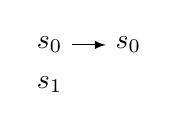
\begin{tikzpicture}[>=latex]
    \node[] (input) {$s_0$};
    \node[right of=input] (output) {$s_0$};
    \node[below of=input,node distance=.5cm] (unused) {$s_1$};
    \draw[->] (input) -- (output);
\end{tikzpicture}
\\
\begin{tikzpicture}[>=latex,node distance=.6cm]
  \node[] (input1) {$s_0$};
  \node[below of=input1] (midway) {};
  \node[below of=midway] (input2) {$s_1$};
  \node[block, right of=midway, node distance=1cm] (T) {$\lift{\pair{\cdot}{\cdot}}$};
  \draw[->] (input1) -| (T);
  \draw[->] (input2) -| (T);
  \node[block, right of=T, node distance=1.5cm] (F) {$\lift{\mbox{snd}}$};
  \node[right of=F, node distance=1cm] (output) {$s_1$};
  \draw[->] (T) -- (F);
  \draw[->] (F) -- (output);
\end{tikzpicture}
&
$\cong$
&
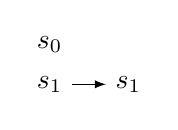
\begin{tikzpicture}[auto,>=latex]
    \node[] (input0) {$s_0$};
    \node[below of=input0,node distance=.5cm] (input1) {$s_1$};
    \node[right of=input1] (output) {$s_1$};
    \draw[->] (input1) -- (output);
\end{tikzpicture}
\\
\begin{tikzpicture}[auto,>=latex]
  \node[] (input) {$p$};
  \node[right of=input, node distance=1.5cm] (midway) {};
  \node[block, above of=midway, node distance=.5cm] (fst) {$\lift{\mbox{fst}}$};
  \node[block, below of=midway, node distance=.5cm] (snd) {$\lift{\mbox{snd}}$};
  \node[block, right of=midway, node distance=1.5cm] (q) {$\lift{\pair{\cdot}{\cdot}}$};
  \node[right of=q] (output) {$p$};
  \draw[->] (input.east) -- ++(2mm,0) |- (fst);
  \draw[->] (input.east) -- ++(2mm,0) |- (snd);
  \draw[->] (fst) -| (q);
  \draw[->] (snd) -| (q);
  \draw[->] (q) -- (output);
\end{tikzpicture}
&
$\cong$
&
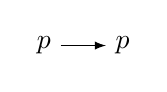
\begin{tikzpicture}[auto,>=latex]
    \node[] (input) {$p$};
    \node[right of=input] (output) {$p$};
    \draw[->] (input) -- (output);
\end{tikzpicture}
\end{tabular}
\end{center}

Pairing and projections allow for switching between pairs of streams and streams of pairs,
whichever is more convenient. For example, instead of a binary operator
$T:\stream{A}\times\stream{B}\to\stream{C}$ we can work with a unary operator
$T^u:\stream{A\times B}\to\stream{C}$ where $T^u(p)=T(\lift{\mbox{fst}}(p),\lift{\mbox{snd}}(p))$
and instead of a unary operator $Q:\stream{A\times B}\to\stream{C}$ we can work with
a binary operator $Q^b:\stream{A}\times\stream{B}\to\stream{C}$ where
$Q^b(s_0,s_1)=Q(\lift{\pair{s_0}{s_1}})$.

\begin{tabular}{m{3.5cm}m{1cm}m{5cm}}
\begin{tikzpicture}[auto,>=latex]
  \node[] (input1) {$s_0$};
  \node[below of=input1,node distance=.5cm] (midway) {};
  \node[below of=midway,node distance=.5cm] (input2) {$s_1$};
  \node[block, right of=midway] (T) {$Q^b$};
  \draw[->] (input1) -| (T);
  \draw[->] (input2) -| (T);
  \node[right of=T] (output) {$s$};
  \draw[->] (T) -- (output);
\end{tikzpicture}
&
$\defn$
&
\begin{tikzpicture}[auto,>=latex]
  \node[] (input1) {$s_0$};
  \node[below of=input1,node distance=.5cm] (midway) {};
  \node[below of=midway,node distance=.5cm] (input2) {$s_1$};
  \node[block, right of=midway] (pair) {$\lift{\pair{\cdot}{\cdot}}$};
  \draw[->] (input1) -| (pair);
  \draw[->] (input2) -| (pair);
  \node[block, right of=pair] (T) {$Q$};
  \node[right of=T] (output) {$s$};
  \draw[->] (pair) -- (T);
  \draw[->] (T) -- (output);
\end{tikzpicture} \\

\begin{tikzpicture}[auto,>=latex]
  \node[] (input) {$p$};
  \node[block, right of=input] (Q) {$T^u$};
  \draw[->] (input) -- (Q);
  \node[right of=Q] (output) {$s$};
  \draw[->] (Q) -- (output);
\end{tikzpicture}
&
$\defn$
&
\begin{tikzpicture}[auto,>=latex]
  \node[] (input) {$p$};
  \node[right of=input, node distance=1.5cm] (midway) {};
  \node[block, above of=midway, node distance=.5cm] (fst) {$\lift{\mbox{fst}}$};
  \node[block, below of=midway, node distance=.5cm] (snd) {$\lift{\mbox{snd}}$};
  \node[block, right of=midway] (q) {$T$};
  \node[right of=q] (output) {$s$};
  \draw[->] (input.east) -- ++(2mm,0) |- (fst);
  \draw[->] (input.east) -- ++(2mm,0) |- (snd);
  \draw[->] (fst) -| (q);
  \draw[->] (snd) -| (q);
  \draw[->] (q) -- (output);
\end{tikzpicture}
\end{tabular}


Given two operators $Q:\stream{A}\to\stream{B}$ and $R:\stream{A}\to\stream{C}$
we define $\lift{\pair{Q}{R}}:\stream{A}\to\stream{B\times C}$ by
$\lift{\pair{Q}{R}}(s)=\lift{\pair{Q(s)}{R(s)}}$. In terms of circuit diagrams:


\begin{tabular}{m{3.5cm}m{.5cm}m{5cm}}
\begin{tikzpicture}[auto,>=latex]
  \node[] (input) {$s$};
  \node[block, right of=input,node distance=1.5cm] (Q) {$\lift{\pair{Q}{R}}$};
  \draw[->] (input) -- (Q);
  \node[right of=Q,node distance=1.5cm] (output) {$o$};
  \draw[->] (Q) -- (output);
\end{tikzpicture}
&
$\cong$
&
\begin{tikzpicture}[auto,>=latex,node distance=.5cm]
  \node[] (input) {$s$};
  \node[block, above right=.1cm and 1cm of input] (a) {$Q$};
  \node[block, below right=.1cm and 1cm of input] (b) {$R$};
  \node[block, right of=input, node distance=2.8cm] (P) {$\lift{\pair{\cdot}{\cdot}}$};
  \node[right of=P,node distance=1cm] (output) {$o$};
  \draw[<-] (a.west) -- ++(-5mm,0) |- (input);
  \draw[<-] (b.west) -- ++(-5mm,0) |- (input);
  \draw[->] (a) -| (P);
  \draw[->] (b) -| (P);
  \draw[->] (P) -- (output);
\end{tikzpicture}
\end{tabular}

We have standard equalities (from category theory) for this construct such
as $\lift{\mbox{fst}}\circ\lift{\pair{Q}{R}}=Q$, similarly for $\mbox{snd}$, and
$\lift{\pair{\lift{\mbox{fst}}\circ W}{\lift{\mbox{snd}}\circ W}} = W$.
These correspond to equivalences of circuits that follow from the simpler ones above.
For example, after substituting the definition of $\pair{Q}{R}$ we have

\begin{tabular}{m{5.5cm}m{1cm}m{2.5cm}}
\begin{tikzpicture}[auto,>=latex,node distance=.5cm]
  \node[] (input) {$s$};
  \node[block, above right=.1cm and 1cm of input] (a) {$R$};
  \node[block, below right=.1cm and 1cm of input] (b) {$S$};
  \node[block, right of=input, node distance=2.8cm] (P) {$\lift{\pair{\cdot}{\cdot}}$};
  \node[block,right of=P,node distance=1.2cm] (F) {$\lift{\mbox{fst}}$};
  \node[right of=F,node distance=1cm] (output) {$o$};
  \draw[<-] (a.west) -- ++(-5mm,0) |- (input);
  \draw[<-] (b.west) -- ++(-5mm,0) |- (input);
  \draw[->] (a) -| (P);
  \draw[->] (b) -| (P);
  \draw[->] (P) -- (F);
  \draw[->] (F) -- (output);
\end{tikzpicture}
&
$\cong$
&
\begin{tikzpicture}[auto,>=latex]
    \node[] (input) {$s$};
    \node[block, right of=input,node distance=1cm] (F) {$R$};
    \node[right of=F] (output) {$o$};
    \draw[->] (input) -- (F);
    \draw[->] (F) -- (output);
\end{tikzpicture}
\end{tabular}


Another useful operator expression notation takes $Q:\stream{A}\to\stream{B}$
and $R:\stream{D}\to\stream{C}$ and combines them into
$Q\times R:\stream{A\times D}\to\stream{B\times C}$ where
$(Q\times R)(p) = \pair{Q(\lift{\mbox{fst}}(p))}{R(\lift{\mbox{snd}}(p))}$.
This corresponds to the following circuit:

\begin{center}
\begin{tikzpicture}[auto,>=latex,node distance=.5cm]
  \node[] (input) {$p$};
  \node[block, above right=0cm and 1cm of input] (a) {$\lift{\mbox{fst}}$};
  \node[block, above right=0cm and 2.5cm of input] (Q) {$Q$};
  \node[block, below right=0cm and 1cm of input] (b) {$\lift{\mbox{snd}}$};
  \node[block, below right=0cm and 2.5cm of input] (R) {$R$};
  \node[block, right of=input, node distance=4cm] (P) {$\lift{\pair{\cdot}{\cdot}}$};
  \node[right of=P,node distance=1cm] (output) {$o$};
  \draw[<-] (a.west) -- ++(-5mm,0) |- (input);
  \draw[<-] (b.west) -- ++(-5mm,0) |- (input);
  \draw[->] (Q) -| (P);
  \draw[->] (R) -| (P);
  \draw[->] (a) -- (Q);
  \draw[->] (b) -- (R);
  \draw[->] (P) -- (output);
\end{tikzpicture}
\end{center}

We also have the following circuit equivalence:

\begin{center}
\begin{tabular}{m{3cm}m{1cm}m{2.5cm}}
\begin{tikzpicture}[auto,>=latex]
  \node[] (input) {$s$};
  \node[block, right of=input] (q) {$Q$};
  \node[above right=0cm and .5cm of q] (a) {$o_0$};
  \node[below right=0cm and .5cm of q] (b) {$o_1$};
  \draw[->] (input) -- (q);
  \draw[->] (q.east) -- ++(2mm,0) |- (a);
  \draw[->] (q.east) -- ++(2mm,0) |- (b);
\end{tikzpicture}
&
$\cong$
&
\begin{tikzpicture}[auto,>=latex]
  \node[] (input) {$s$};
  \node[block, above right=0cm and .5cm of input] (q0) {$Q$};
  \node[block, below right=0cm and .5cm of input] (q1) {$Q$};
  \node[right of=q0] (output0) {$o_0$};
  \node[right of=q1] (output1) {$o_1$};
  \draw[->] (input.east) -- ++(2mm,0) |- (q0);
  \draw[->] (input.east) -- ++(2mm,0) |- (q1);
  \draw[->] (q0) -- (output0);
  \draw[->] (q1) -- (output1);
\end{tikzpicture}
\end{tabular}
\end{center}

\val{Should this one be here? It is unrelated to products.
Let em email you a proposal for organizing these equivalences and definitions}


Lifting functions on values and composing stream operators results in a very simple, yet limited, programming language on streams.
We next introduce operators that ``shift'' streams in time.
These will be instrumental for enriching the language.

\subsection{Streams over abelian groups}\label{sec:abelian}

For the rest of the technical development we will require the set of values $(A, +, 0, -)$
for any stream $\stream{A}$ to form a commutative group.

We denote by $0_{\stream{A}}$ (or simply $0$ when the type is clear) the stream that consist of the special
value 0 at each time moment: $0_{\stream{A}} \in \stream{A}$, $\forall t \in \N . 0_{\stream{A}}[t] \defn 0_A$.

\subsubsection{Delays and time-invariance}\label{sec:delay}

\begin{definition}[Delay]
The \defined{delay operator}\footnote{The name $\zm$
comes form the DSP literature, and it is related to the z-transform.} emits an output stream that is
the input stream delayed by one element: $\zm_A: \stream{A} \to \stream{A}$ defined by:
$$
\zm_A(s)[t] \defn  \begin{cases}
s[t - 1] & \text{when}~t\geq1\\
0_A      & \text{when}~t=0
\end{cases}
$$

We often omit the type parameter $A$, and write just $\zm$.
We denote by $z^{-k}$ the composition of $\zm$
with itself $k$ times (delay by $k$ time units).
\end{definition}

\begin{center}
\begin{tikzpicture}[auto,node distance=1cm,>=latex]
    \node[] (input) {$i$};
    \node[block, right of=input] (z) {$\zm$};
    \node[right of=z] (output) {$o$};
    \draw[->] (input) -- (z);
    \draw[->] (z) -- (output);
\end{tikzpicture}
\end{center}

For example, the delay of the $\id$ stream is $\zm(\id)$, containing
the sequence of values $\sv{0 0 1 2 3}$.

\qquad

The following definition applies to stream operators of
any number of arguments but to keep the notation simpler we formulate it only for binary operators.

\begin{definition}[Time invariance]
A stream operator $T: \stream{A_0}\times\stream{A_1} \to \stream{B}$ is \defined{time-invariant} if it commutes with the delay operator $\zm$, that is, \\
$T(\zm(s_0),\zm(s_1)) = \zm(T(s_0,s_1))$ for any $s_0 \in \stream{A_0}, s_1 \in \stream{A_1}$.
\end{definition}
In other words, $T$ is time-invariant if and only if the following two circuits are equivalent:

\begin{center}
\begin{tabular}{m{3cm}m{.5cm}m{3cm}}
\begin{tikzpicture}[auto,node distance=.5cm,>=latex]
  \node[] (input1) {$s_0$};
  \node[below of=input1] (midway) {};
  \node[below of=midway] (input2) {$s_1$};
  \node[block, right of=midway, node distance=1cm] (T) {$T$};
  \node[block, right of=T,node distance=1cm] (z) {$\zm$};
  \node[right of=z,node distance=1cm] (output) {$o$};
  \draw[->] (input1) -| (T);
  \draw[->] (input2) -| (T);
  \draw[->] (T) -- (z);
  \draw[->] (z) -- (output);
\end{tikzpicture}
&
$\cong$
&
\begin{tikzpicture}[auto,node distance=.5cm,>=latex]
  \node[] (input1) {$s_0$};
  \node[below of=input1] (midway) {};
  \node[below of=midway] (input2) {$s_1$};
  \node[block, right of=input1, node distance=1cm] (z1) {$\zm$};
  \node[block, right of=input2, node distance=1cm] (z2) {$\zm$};
  \node[block, right of=midway, node distance=2cm] (T) {$T$};
  \node[right of=T,node distance=1cm] (output) {$o$};
  \draw[->] (input1) -- (z1);
  \draw[->] (input2) -- (z2);
  \draw[->] (z1) -| (T);
  \draw[->] (z2) -| (T);
  \draw[->] (T) -- (output);
\end{tikzpicture}
\end{tabular}
\end{center}

It is straightforward to check that the composition
of any number of time-invariant operators of any number of arguments
is time invariant. Similarly, the delay operators $z^{-k}$ as well as the
pairing and projection operators are time-invariant.
In this framework we only deal with time-invariant operators.

\begin{definition}
We say that a function between groups $f: A \to B$ has the \defined{zero-preservation
property} iff $f(0_A) = 0_B$.  We write $\zpp{f}$.  This property generalizes to functions
with multiple inputs: e.g., $g: A \times B \to C$ where $A, B, C$ are groups.  $\zpp{g}$
iff $g(0_A, 0_B) = 0_C$.
\end{definition}

\begin{proposition}
A lifted operator $\lift{f}$ is time-invariant iff $\zpp{f}$.
\end{proposition}

Notice that it is easy to construct operators that are not time-invariant.
Consider the ``constant 1'' function: $c_1: \N \rightarrow \N$, defined by
$c_1(x) = 1, \forall x \in \N$.
The stream operator defined by $\lift{c_1}: \stream{N} \rightarrow \stream{N}$
produces a stream containing only the constant value 1: $c_1(s)[t] = 1,
\forall s \in \stream{N}, t \in \N$.  The stream operator $\lift{c_1}$
is \emph{not} time-invariant, since it does not have the zero preservation property.

\begin{comment}
\begin{definition}
We call an operator $o: \stream{A} \rightarrow \stream{B}$ over streams
\defined{memoryless} if it can be produced by lifting a function pointwise, i.e.,
there exists a function $f: A \rightarrow B$ such that
$\forall s \in \stream{A} . o(s)[t] = f(s[t])$.

\begin{example}
Whatever definition we give to ``memoryless'' it should be the case that
any memoryless operator is causal.
\end{example}
\end{definition}
\end{comment}

\subsection{Causal and strict operators}\label{sec:causal}

For notation simplicity we again give the next definition only for unary operators;
it extends naturally to binary operators through the use of pairing as shown above.

\begin{definition}[Causality]
A stream operator, $S:\stream{A}\to\stream{B}$,
is \defined{causal} when for any $s,s'\in\stream{A}$,
and all times $t$ we have
$$
(\forall i\leq t~s[i]=s'[i]) ~~\text{implies}~~ S(s)[t]=S(s')[t]
$$
\end{definition}

Note that all operators produced by lifting scalar functions are causal.
$\zm$ is causal.  All \dbsp operators are causal.

\begin{definition}[Cutting]
\defined{Cutting} the stream $s \in \stream{A}$ at time $t \in \N$ produces a stream
$$
(\cut{s}{t})[i] \defn  \begin{cases}
                      s[i] &\text{if}~i\leq t\\
                      0_A  &\text{if}~i>t
                      \end{cases}
$$
\end{definition}
For example, cutting the stream $\id$ at time 2 gives the stream $\cut{\id}{2}$
composed of the sequence $\sv{0 1 2 0 0}$.

Note that $\cut{\cut{s}{t_1}}{t_2}=\cut{s}{\min(t_1,t_2)}$. It follows that
$\cut{\cut{s}{t_1}}{t_2}=\cut{\cut{s}{t_2}}{t_1}$ (cutting is commutative) and
$\cut{\cut{s}{t}}{t}=\cut{s}{t}$, (cutting at time $t$ is idempotent).
Cutting, however, is \textbf{not} time-invariant.  Cutting is not
used as a \dbsp operator, it is just a mathematical tool that we will use to
reason about the behavior of the circuits we build.

\begin{lemma}
\label{lemma-causal-characterization}
The following are equivalent for a binary stream operator $T$
\begin{enumerate}
\item[(i)] $T$ is causal
\item[(ii)] $\forall s_1,s_2$ and $t$  we have $\cut{T(s_1,s_2)}{t} ~=~ \cut{T(\cut{s_1}{t},\cut{s_2}{t})}{t}$~.
\end{enumerate}
\end{lemma}
Using part (ii) it follows immediately that the composition
of any number of causal operators of any number of arguments is causal.
Moreover, using also the commutativity and idempotence of cutting, it follows that
for any $t$ the operator $\lambda s.\cut{s}{t}$ is itself causal.

\begin{definition}[zero almost everywhere]\label{def:zae}
We say that a stream $s$ is \defined{zero almost-everywhere} if there exists a time $t_0 \in \N$
s.t. $\cut{s}{t_0} = s$.
\end{definition}

%Such a stream can be described entirely by providing its prefix up to time $t_0$,
%a finite stream.
We denote the set of streams over $A$ that are zero almost everywhere
by $\streamf{A}$.

\begin{definition}[Strictness]
A stream operator, $F:\stream{A}\to\stream{B}$
is \defined{strictly causal} (abbreviated \textbf{strict})
if for any $s,s'\in\stream{A}$ and all times $t$ we have
$$
(\forall i<t . s[i]=s'[i]) ~~\text{implies}~~ F(s)[t]=F(s')[t]
$$
\end{definition}

In particular, $F(s)[0] = 0_B$ is the same for all inputs $s \in \stream{A}$.
Strict operators are of course causal. Note that lifted stream operators,
while causal, in general are \emph{not} strict.

It can be immediately checked that the operator $\zm$
(in fact, $z^{-k}$ for any positive integer $k$)
is strict.
In this text $\zm$ is the only primitive strict operator used.

\begin{definition}[Strict cutting]
\defined{Strictly cutting} the stream $s \in \stream{A}$ at time $t \in \N$ produces the stream
$$
(\scut{s}{t})[i] \defn  \begin{cases}
                      s[i] &\text{if}~i< t\\
                      0_A  &\text{if}~i\geq t
                      \end{cases}
$$
\end{definition}

$\scut{s}{0}$ is the stream $0_{\stream{A}}$ that is $0_A$ at all times.
Note also that $\scut{s}{t+1} =\cut{s}{t}$.


Analogously to Lemma~\ref{lemma-causal-characterization} an operator $F: \stream{A} \to \stream{B}$ is strict iff for any $s$ and $t$ we have
$$
\cut{F(s)}{t} ~=~ \cut{F(\scut{s}{t})}{t}
$$
In particular, $F(s)[0] = F(0_{\stream{A}})[0]$ and
$F(s)[t+1]=F(\cut{s}{t})[t+1]$.  Note the different zeros in $F(0_{\stream{A}})[0]$:
it features both the stream $0_{\stream{A}} \in \stream{A}$, consisting of the group element $0_A$
at each time moment, and the time moment $0$.

The next proposition shows the importance of strict operators.
\begin{proposition}
\label{prop-unique-fix}
For any strict operator $F: \stream{A} \to \stream{A}$ the equation ~$\alpha=F(\alpha)$~ has a unique
solution $\alpha \in \stream{A}$.  In other words, every strict operator has a unique fixed point,
which we denote by $\fix{\alpha}{F(\alpha)}$.
\end{proposition}
%\leonid{Usually fixed-points require some monotonicity.  What is it here?}

\begin{proof}
Define the solution (the fixed point) by recurrence:
\begin{eqnarray*}
\alpha[0] & = &  F(\alpha)[0]=F(0_{\stream{A}})[0]\\
\alpha[t+1] & = & F(\alpha)[t+1]=F(\cut{\alpha}{t})[t+1]
\end{eqnarray*}
The second equality defines $\alpha[t+1]$ in terms of $\alpha[0],\ldots,\alpha[t]$.
Uniqueness follows by strong induction.

\qquad
\end{proof}

We will apply the previous proposition to operators obtained by composing strict and causal ones.
\begin{lemma}
\label{lemma-causal-strict}
Let $k\geq 2$. If $F$ is strict and the $k$-ary $T$ operator is causal, then for any
fixed $s_0,\ldots,s_{k-2}$ the operator
$\lambda\alpha.T(s_0,\ldots,s_{k-2},F(\alpha))$ is strict.
\end{lemma}

\begin{proof} We show the case $k=2$.
This operator is described by the following diagram with a ``feedback loop'':

\begin{center}
\begin{tikzpicture}[>=latex]
    \node[] (input) {$s$};
    \node[block, right of=input] (f) {$T$};
    \node[right of=f, node distance=1.5cm] (output) {$\alpha$};
    \node[block, below of=f, node distance=.8cm] (z) {$F$};
    \draw[->] (input) -- (f);
    \draw[->] (f) -- node (mid) {} (output);
    \draw[->] (mid.center) |-  (z);
    \draw[->] (z.west) -- ++(-.3,0) |- ([yshift=1mm]f.south west);
\end{tikzpicture}
\end{center}
\begin{eqnarray*}
\cut{T(s,F(\alpha))}{t} & = & \cut{T(\cut{s}{t},\cut{F(\alpha)}{t})}{t}\\
                   & = & \cut{T(\cut{s}{t},\cut{F(\scut{\alpha}{t})}{t})}{t}\\
                   & = & \cut{T(s,F(\scut{\alpha}{t}))}{t}
\end{eqnarray*}
\qquad
\end{proof}


\begin{corollary}
\label{cor-fix-cut}
For strict $F$ we have
$$
\cut{(\fix{\alpha}{F(\alpha)})}{t} ~=~  \fix{\alpha}{(\cut{F(\alpha)}{t})}
$$
\end{corollary}
\begin{proof}
Since cutting itself is a causal operator, it follows from Lemma~\ref{lemma-causal-strict} that $\lambda\alpha.(\cut{F(\alpha)}{t})$ is strict
so Proposition~\ref{prop-unique-fix} applies and $\fix{\alpha}{(\cut{F(\alpha)}{t})}$
is well-defined.

If we let $\alpha$ be the solution of $\alpha=F(\alpha)$ then, by uniqueness, it suffices to show that $\beta=\cut{\alpha}{t}$ satisfies
the equation $\beta=\cut{F(\beta)}{t}$. Indeed, since $F$ is in particular causal
$$
\cut{\alpha}{t} = \cut{F(\alpha)}{t} = \cut{F(\cut{\alpha}{t})}{t}
$$


\qquad
\end{proof}

\begin{corollary}\label{feedback-semantics}
\label{cor-loop}
Let $k\geq1$. If $F: \stream{A} \to \stream{A}$ is strict and $(k+1)$-ary $T$ is causal then the $k$-ary
operator $Q(s_0,\ldots,s_{k-1})=\fix{\alpha}{T(s_0,\ldots,s_{k-1},F(\alpha))}$~ is well-defined and causal.
If, moreover, $F$ and $T$ are time-invariant then so is $Q$.
\end{corollary}
\begin{proof} We show the case $k=1$.
The well-definedness of $Q$ follows by applying, for each $s$, Proposition~\ref{prop-unique-fix}
to the operator
$\lambda\alpha.T(s,F(\alpha))$ which is strict by Lemma~\ref{lemma-causal-strict}.
For future reference it might be useful to state the defining recurrence for a stream $\alpha$
produced by this operator, that is, $\alpha=Q(s)$:
\begin{eqnarray*}
\alpha[0] & = &  T(s,F(0_{\stream{A}}))[0]\\
\alpha[t+1] & = & T(s,F(\cut{\alpha}{t}))[t+1]
\end{eqnarray*}
To prove that $Q$ is causal we could use this recurrence and induction. Instead
we use the causality of $T$ and the idempotence of cutting in conjunction with
Corollary~\ref{cor-fix-cut} as follows:
\begin{eqnarray*}
\cut{Q(s)}{t} & = &  \cut{(\fix{\alpha}{T(s,F(\alpha))})}{t}\\
         & = &  \fix{\alpha}{\cut{(T(s,F(\alpha))}{t})}~~~~~~~~~~~~\mbox{(Corollary~\ref{cor-fix-cut})}\\
         & = &  \fix{\alpha}{(\cut{T(\cut{s}{t},\cut{F(\alpha)}{t})}{t})}~~~~~~\mbox{(Causality of $T$)}\\
         & = &  \fix{\alpha}{(\cut{T(\cut{\cut{s}{t}}{t},\cut{F(\alpha)}{t})}{t})}~~~\mbox{(Idempotence of cutting)}\\
         & = &  \fix{\alpha}{\cut{(T(\cut{s}{t},F(\alpha))}{t})}~~~~~~~~~~\mbox{(Causality of $T$)}\\
         & = & \cut{(\fix{\alpha}{T(\cut{s}{t},F(\alpha))})}{t}~~~~~~~~~~\mbox{(Corollary~\ref{cor-fix-cut})}\\
         & = & \cut{Q(\cut{s}{t})}{t}
\end{eqnarray*}
For time-invariance we observe that if $\alpha=T(s,F(\alpha))$ then $\zm(\alpha)= \zm(T(s,F(\alpha)))=T(\zm(s),\zm(F(\alpha))=
T(\zm(s),F(\zm(\alpha)))$. It follows that $\beta=\zm(\alpha)$ satisfies the equation $\beta=T(\zm(s),F(\beta))$ so,
by uniqueness of the fixed point $Q(\zm(s))=\zm(Q(s))$.
\end{proof}



Ostensibly this covers a form of straightforward recursion but how about mutual recursion? For instance, assuming $T_1,T_2$ are causal and $F_1,F_2$ are strict we wish to claim that the following is well defined: $Q_1(s_1,s_2)=\alpha_1$ and $Q_2(s_1,s_2)=\alpha_2$ where:
\begin{eqnarray*}
\alpha_1 & = & T_1(s_1,F_1(\alpha_2))~~~~~\mbox{and}\\
\alpha_2 & = & T_2(s_2,F_2(\alpha_1))
\end{eqnarray*}
Here is the corresponding diagram:

\begin{center}
\begin{tikzpicture}[>=latex]
  \node[] (i1) {$s_1$};
  \node[below of=i1, node distance=.7cm] (i2) {$s_2$};
  \node[block, right of=i1, node distance=1.5cm] (t1) {$T_1$};
  \node[block, right of=i2, node distance=1.5cm] (t2) {$T_2$};
  \node[right of=t1, node distance=1.5cm] (o1) {$\alpha_1$};
  \node[right of=t2, node distance=2cm] (o2) {$\alpha_2$};

  \node[block, below of=t2] (f1) {$F_2$};
  \node[block, below of=f1, node distance=.7cm] (f2) {$F_1$};

  \draw[->] (i1) -- (t1);
  \draw[->] (i2) -- (t2);
  \draw[->] (t1) -- node (m1) {} (o1);
  \draw[->] (t2) -- node (m2) {} (o2);
  \draw[->] (m1.center) |- (f1);
  \draw[->] (m2.center) |- (f2);

  \draw[->] (f1.west) -- ++(-.3,0) |- ([yshift=1mm]t2.south west);
  \draw[->] (f2.west) -- ++(-.4,0) |- ([yshift=1mm]t1.south west);

\end{tikzpicture}
\end{center}

In section~\ref{sec:pairing} we defined constructions on pairs of streams/streams of pairs.
%that we defined in Section~\ref{sec:cartesian}
In particular, for binary $T_1:\stream{A_1}\times\stream{B_1}\to\stream{C_1}$ and
binary $T_2:\stream{A_2}\times\stream{B_2}\to\stream{C_2}$
let
\val{For binary operators we should have defined $\times$ this way in section~\ref{sec:pairing} ...
Also, in the def of $T_1\times T_2$ note that I did not put a lift in front of the stream pairing operator on the RHS. }
binary $T_1\times T_2:\stream{A_1\times A_2}\times\stream{B_1\times B_2}\to\stream{C_1\times C_2}$
$$
[T_1\times T_2](p,q) = \pair{T_1(\lift{\mbox{fst}}\circ p,\lift{\mbox{fst}}\circ q)}
{T_2(\lift{\mbox{snd}}\circ p,\lift{\mbox{snd}}\circ q)}
$$
In addition, we use $F_1\times F_2:\stream{C_1\times C_2}\to\stream{B_1\times B_2}$ as defined in section~\ref{sec:pairing}. Let also $\mbox{swap}: C_1\times C_2 \to C_2 \times C_1$
be the operator that swaps the components of a pairs (obtained by pairing the second projection
with the third.
\begin{proposition}
If $T_1$ and $T_2$ are causal then $T_1\circ T_2$ is causal. If $F_1$ and $F_2$ are strict then
$(F_1\times F_2)\circ\lift{\mbox{swap}}$ is strict.
\end{proposition}
The circuit above is equivalent to the following (when composed with projections of outputs
and pairing of inputs:

\begin{center}
\begin{tikzpicture}[>=latex]
    \node[] (input) {$s$};
    \node[block, right of=input, node distance=2cm] (f) {$T_1\times T_2$};
    \node[right of=f, node distance=3cm] (output) {$\alpha$};
    \node[block, below of=f] (z) {($F_1\times F_2)\circ\lift{\mbox{swap}}$};
    \draw[->] (input) -- (f);
    \draw[->] (f) -- ++(2,0) node (mid) {} -- (output);
    \draw[->] (mid.center) |-  (z);
    \draw[->] (z.west) -- ++(-.3,0) |- ([yshift=1mm]f.south west);
\end{tikzpicture}
\end{center}

In other words,
we can apply Corollary~\ref{feedback-semantics} to the causal operator $T_1\times T_2$
and the strict operator $F_1\times F_2$ and obtain $Q_1$ and $Q_2$ from
$$
\fix{\alpha}{[T_1\times T_2](\pair{s_1}{s_2},[F_1\times F_2](\mbox{swap}(\alpha)))}
$$
by further projecting, where $\alpha$ is a variable of type pair of streams and $\overline{\alpha}$
swaps the two components.


\val{We should state this a some kind of corollary to the corollary.}
\mihai{This becomes complicated for $n$-way mutual recursion, you have a quadratic number of edges.
Maybe it's simpler to assume that all of them use all of the alphas, and the projection to a subset
is part of $T$ if needed.}



\subsection{Streams as an abelian group}\label{sec:abelianstreams}

Remember that we require the elements of a stream to come from an Abelian group:
$(A,+,0,-)$.  This structure also lifts to streams:

\begin{proposition}
$(\stream{A},+,0_{\stream{A}},-)$ (with the operations lifted pointwise in time)
is also an abelian group. Moreover, lifting a group homomorphism produces
a stream operator that is itself a group homomorphism.
In addition, when $A$ and $B$ are abelian groups there is a standard abelian group structure
on $A\times B$, with the zero $0_{A \times B}$ the pair $\pair{0_A}{0_B}$.
\end{proposition}


\begin{definition}[linear]
If $A$ and $B$ are abelian groups, we call
a function $f: A \rightarrow B$ \defined{linear} if it is a group homomorphism, that is,
$f(a+b)=f(a)+f(b)$ (and therefore $f(0_A)=0_B$ and $f(-a)=-f(a)$); thus $\zpp{f}$.
\end{definition}

We use the abbreviation LTI for a stream operator that is linear and time-invariant.

Lifting a linear function $f: A \to B$ produces a stream operator $\lift{f}$ that is causal and LTI.
It follows that stream addition and negation are causal and LTI.
$\zm$ is LTI, (and so is $z^{-k}$ for all $k$).

\begin{definition}[multilinear, bilinear]
We define \defined{multilinear} (in particular, \defined{bilinear}) functions as functions (between groups) of multiple
arguments that are linear separately in each argument (that is, if we fix all but one argument,
the resulting function is linear in that argument.  In other words, the function distributes over addition):
e.g., for $g: A_0 \times A_1 \to B, \forall a, b \in A_0, c, d \in A_1 . g(a+b, c) = g(a, c) + g(b, c)$,
and $g(a, c+d) = g(a, c) + g(c, d)$.
\end{definition}

Multiplication over $\Z$ is a bilinear function.  For a bilinear function $g$ we have $\zpp{g}$.

This definition extends to stream operators.
Lifting any bilinear function $g: A \times B \to C$ produces a bilinear stream operator $\lift{g}$.
An example bi-linear operator over $\stream{\Z}$ is the lifted integer multiplication:
$T: \stream{\Z} \times \stream{\Z} \to \stream{\Z}, T(a, b)[t] = a[t]\cdot b[t]$.

The composition of multilinear operators with linear operators is multilinear (since homomorphisms compose).
Since linear and bilinear functions have the zero-preservation property,
lifted linear and bilinear functions operators are all time-invariant.

\begin{proposition}
The composition of a bilinear operator followed by a linear operator is a bilinear operator.
\end{proposition}
\begin{proof}
Consider $T: \stream{A} \times \stream{B} \to \stream{C}$ a bilinear operator, and
$S: \stream{C} \to \stream{C}$, a linear operator.  Let us compute $S(T(a+b, c)) = S(T(a, c) + T(b, c)) =
S(T(a, c)) + S(T(b, c)).$  Thus $S \circ T$ is bilinear.
\end{proof}

Lifting a multilinear operator $A_1\times\cdots\times A_n \rightarrow B$ produces a multilinear, time-invariant stream operator. Although combining pairs (tuples) of
streams into stream of pairs (tuples) can be useful
we must note a distinction (well understood in algebra):
we have seen that we can use instead of a binary stream operator
$T:\stream{A}\times\stream{B}\to\stream{C}$ a unary version that acts on streams of pairs
$T^u:\stream{A\times B}\to\stream{C}$ where $T^u\pair{a}{b}=T(a,b)$. However, in contrast to causality,
there is, in general, no relation between the linearity. %\footnote{Recall the
%abelian group structure on $A\times B$.} of $T^u$ and the bilinearity of $T$.
%\mihai{I still think that the motivation for this statement is unclear.}

In traditional signal processing most operators are LTI but in our development
we will use some important non-linear ones.

The ``feedback-loop'' operators defined by recurrence in Corollary~\ref{cor-loop},
e.g., $\lambda s.\fix{\alpha}{T(s,F(\alpha))}$ are, in general, not (multi)linear.
\val{Counterexample even for bilinear $S$ and $\lambda s_1.\lambda s_2.\fix{\alpha}{S(s_1,s_2+\zm(\alpha))}$? Possibly $S$ is join NOT followed by distinct?}
However, multilinearity holds in important particular cases,
as shown in the following proposition:

\begin{proposition}
\label{prop-rec-linear}
Let $S$ be a unary causal, LTI operator. Then, the
operator $Q(s)=\fix{\alpha}{S(s+\zm(\alpha))}$~ is well-defined and LTI.
\end{proposition}
\mihai{Notice that this is a very nice kind of recursion, a tail-recursion.}

\begin{center}
\begin{tikzpicture}[>=latex]
    \node[] (input) {$s$};
    \node[block, shape=circle, right of=input, inner sep=0pt] (plus) {$+$};
    \node[block, right of=plus] (Q) {$S$};
    \node[right of=Q, node distance=1.5cm] (output) {$\alpha$};
    \node[block, below of=Q, node distance=.8cm] (z) {$\zm$};
    \draw[->] (input) -- (plus);
    \draw[->] (plus) -- (Q);
    \draw[->] (Q) -- node (mid) {} (output);
    \draw[->] (mid.center) |-  (z);
    \draw[->] (z) -| (plus);
\end{tikzpicture}
\end{center}

\begin{proof} Since $S$ and the addition operator
are causal and $\zm$ is strict, Proposition~\ref{prop-unique-fix} applies,
for each $s$, to the operator
$\lambda\alpha.S(s+\zm(\alpha))$ which is strict by Lemma~\ref{lemma-causal-strict}.
Thus $Q$ is well-defined.

Fix streams $s_0$ and $s_1$. Let $\alpha_0$
be the unique solution of $\alpha_0=S(s_0+\zm(\alpha_0))$ and
$\alpha_1$ be the unique solution of $\alpha_1=S(s_1+\zm(\alpha_1))$.
Then $\alpha=\alpha_0+\alpha_1$ is the unique solution of
$\alpha=Q(s_0+s_1+\zm(\alpha))$. This is justified by adding the equations
and using the linearity of $S$ and the linearity of $\zm$.
\end{proof}

\begin{proposition}
If $T$ is binary causal, $G$ is unary causal, and $F$ is unary strict then:
$$
\fix{\alpha}{G(T(s,F(\alpha)))} = G(\fix{\beta}{T(s,F(G(\beta)))})
$$

\noindent In terms of diagrams:

\begin{tabular}{m{4cm}m{1cm}m{5cm}}
\begin{tikzpicture}[>=latex]
    \node[] (input) {$s$};
    \node[block, right of=input] (t) {$T$};
    \node[block, right of=t] (g) {$G$};
    \node[right of=g, node distance=1.5cm] (output) {$o$};
    \node[block, below of=t, node distance=.8cm] (f) {$F$};
    \draw[->] (input) -- (t);
    \draw[->] (t) -- (g);
    \draw[->] (g) -- node (mid) {} (output);
    \draw[->] (mid.center) |-  (f);
    \draw[->] (f.west) -- ++(-.3,0) |- ([yshift=1mm]t.south west);
\end{tikzpicture}
&
$\cong$
&
\begin{tikzpicture}[>=latex]
    \node[] (input) {$s$};
    \node[block, right of=input, node distance=2cm] (t) {$T$};
    \node[block, right of=t, node distance=1.5cm] (g) {$G$};
    \node[right of=g] (output) {$o$};
    \node[block, below of=t, node distance=.8cm] (g1) {$G$};
    \node[block, left of=g1] (f) {$F$};
    \draw[->] (input) -- (t);
    \draw[->] (t) -- node (mid) {} (g);
    \draw[->] (g) -- (output);
    \draw[->] (mid.center) |-  (g1);
    \draw[->] (g1) -- (f);
    \draw[->] (f.west) -- ++(-.3,0) |- ([yshift=1mm]t.south west);
\end{tikzpicture}
\end{tabular}
\end{proposition}

\begin{proof}
For the second fixpoint to exist we need to show that $F\circ G$ is strict.
Once we do that, by uniqueness of solutions, it remains to show that if $\beta$ is a solution to  $\beta=T(s,F(G(\beta))$ then $\alpha=G(\beta)$ is a solution to
$\alpha=G(T(s,F(\alpha))$ which is immediate by applying $G$ to the first equation.
So let's prove that $F\circ G$ is strict. For $t>0$ we have
\begin{eqnarray*}
\cut{F(G(s))}{t} & = & \cut{F(\scut{G(s)}{t})}{t}~~~~~\mbox{($F$ strict)}\\
                 & = & \cut{F(\cut{G(s)}{t-1})}{t}~~~~~\mbox{($t\geq1$)}\\
                 & = & \cut{F(G(\cut{s}{t-1}))}{t}~~~~~\mbox{($G$ causal)}\\
                 & = & \cut{F(G(\scut{s}{t}))}{t}
\end{eqnarray*}
For $t=0$ just observe that $F(G(s))[0]$ is the same for any $G(s)$ therefore for any $s$.
Note that if $G$ is not causal then $F\circ G$ is not strict and the fixed point may not exist.
\end{proof}


\subsection{Differentiation and Integration}

\begin{definition}[Differentiation]
The \defined{differentiation operator} $\D_{\stream{A}} : \stream{A} \to \stream{A}$ is defined by:
$$
\D_{\stream{A}}(s) \defn s - \zm(s)
$$
\end{definition}
We generally omit the type, and write just $\D$ when the type can be inferred from the context.

The value of $\D(s)$ (at time $t$) is the difference
between  the current (time $t$) value of $s$ and the previous (time $t-1$) value of $s$.

As an example, applying $\D$ to the stream $\id$ gives a result a
stream $\D(\id)$ containing the values $\sv{0 1 1 1 1}$.

\begin{center}
\begin{tikzpicture}[auto,>=latex,node distance=1cm]
    \node[] (input) {$s$};
    \node[block, shape=circle, right of=input, inner sep=0pt,node distance=2cm] (plus) {$+$};
    \node[right of=plus] (output) {$\D(s)$};
    \draw[draw,->] (input) -- node (i) {} (plus);
    \node[block, below of=i, node distance=.8cm] (z) {$\zm$};
    \node[block, shape=circle, right of=z, inner sep=0pt] (minus) {$-$};
    \draw[->] (plus) -- (output);
    \draw[->] (i) -- (z);
    \draw[->] (z) -- (minus);
    \draw[->] (minus) -- (plus);
\end{tikzpicture}
\end{center}

\begin{proposition}
\label{prop-diff-properties}
The differentiation operator $\D$ is causal and LTI.
\end{proposition}
\begin{proof}
Follow from definition using the properties of subtraction and delay.
\end{proof}

The integration operator ``reconstitutes'' a stream from its changes:

\begin{definition}[Integration]
The \defined{integration operator}  $\I_{\stream{A}} : \stream{A} \to \stream{A}$
is defined by $\I_{\stream{A}}(s) \defn \lambda s . \fix{\alpha}{(s + \zm(\alpha))}$.
\end{definition}

\noindent
We also generally omit the type, and write just $\I$.
This is the construction from Proposition~\ref{prop-rec-linear}
using the identity function for $S$.

\begin{center}
\begin{tikzpicture}[auto,>=latex]
    \node[] (input) {$s$};
    \node[block, shape=circle, right of=input, inner sep=0pt] (plus) {$+$};
    \node[right of=plus, node distance=2cm] (output) {$\I(s)$};
    \node[block, below of=plus, node distance=.8cm] (z) {$z^{-1}$};
    \draw[draw,->] (input) -- (plus);
    \draw[->] (plus) -- node (o) {} (output);
    \draw[->] (o) |- (z);
    \draw[->] (z) -- (plus);
\end{tikzpicture}
\end{center}

As an example, applying $\I$ to the $\id$ stream gives as result
a stream $\I(\id)$ composed of the values $\sv{0 1 3 6 10}$.

\begin{proposition}~\label{iprop}
$\I(s)$ is the discrete (indefinite) integral applied to the stream $s$:
$\I(s)[t] = \sum_{i \leq t} s[i]$.
\end{proposition}
\begin{proof} The recurrence from Corollary~\ref{cor-loop} specializes to
\begin{eqnarray*}
\alpha[0]  & = & s[0]\\
\alpha[t+1] & = & \alpha[t] + s[t+1]
\end{eqnarray*}
and it's straightforward to check that $\alpha[t]= \sum_{i \leq t} s[i]$ satisfies
it.
\end{proof}

\begin{proposition}[Properties of $\I$]
\label{prop-integ-properties}
The integration operator $\I$ is causal and LTI.
\end{proposition}
\begin{proof}
By Proposition~\ref{iprop} these properties follow from Corollary~\ref{cor-loop} and Proposition~\ref{prop-rec-linear}.  They also be checked directly using
the definition by summation.
\end{proof}


\begin{theorem}[Inversion]
\label{inverses}
The integration and differentiation operators are inverse to each other. Equivalently, for any streams
$\alpha$ and $s$ we have $\alpha=\I(s)$ iff $\D(\alpha)=s$.
\end{theorem}
\begin{proof}
This can be shown directly from the definitions, for example
  $$
  \begin{aligned}
  \D(\I(s))[t] &= (\I(s) - \zm(\I(s)))[t] & \mbox{definition of }\D \\
  &= \sum_{k \leq t} s[k] - \zm(\sum_{k \leq t} s[k])[t] &
  \mbox{Property }~\ref{prop-integ-properties} \\
  &= \sum_{k \leq t} s[k] - \sum_{k \leq t-1} s[k] & \mbox{definition of }\zm \\
  &= s[t]
  \end{aligned}
  $$
(and similarly we can show that $\I(\D(s'))[t] =s'[t]$).

Alternatively, the equivalent form of the theorem follows from Proposition~\ref{iprop} by observing that
$\D(\alpha)=s$ iff $\alpha=s+\zm(\alpha)$ which is the equation on streams that defines $\alpha=\I(s)$.
%A third proof, bringing some new insights, is given in Section~\ref{sec:ztransform}.
\end{proof}

So we have the following circuit equivalence:

\noindent
\begin{tabular}{m{3.5cm}m{.7cm}m{1.5cm}m{.7cm}m{3.5cm}}
\begin{tikzpicture}[auto,>=latex]
    \node[] (input) {$s$};
    \node[block, right of=input] (I) {$\I$};
    \node[block, right of=I] (D) {$\D$};
    \node[right of=D] (output) {$o$};
    \draw[->] (input) -- (I);
    \draw[->] (I) -- (D);
    \draw[->] (D) -- (output);
\end{tikzpicture}
     &
     $\cong$
     &
\begin{tikzpicture}[auto,>=latex]
    \node[] (input) {$s$};
    \node[right of=input] (output) {$o$};
    \draw[->] (input) -- (output);
\end{tikzpicture}
     &
     $\cong$
     &
\begin{tikzpicture}[auto,>=latex]
    \node[] (input) {$s$};
    \node[block, right of=input] (D) {$\D$};
    \node[block, right of=D] (I) {$\I$};
    \node[right of=I] (output) {$o$};
    \draw[->] (input) -- (D);
    \draw[->] (D) -- (I);
    \draw[->] (I) -- (output);
\end{tikzpicture}
\end{tabular}


Since $\I$ and $\D$ are inverse to each other they are both bijections on streams.

If we define addition of pairs as adding the pair elements pointwise, we also have
the following identities: $\I(\pair{s}{t}) = \pair{\I(s)}{\I(t)}$ and $\D(\pair{s}{t}) = \pair{\D(s)}{\D(t)}$.

\paragraph{Observation}
It is a standard algebraic fact that the inverse of a homomorphism is also a homomorphism.
Thus, $\I$ is linear iff $\D$ is linear. Another immediate consequence of this theorem is that $\I$ is time-invariant iff
$\D$ is time-invariant.
%\val{I believe but I have not checked that}
%\mihai{It looks right}
Moreover $\I$ is causal iff
$\D$ is causal. Therefore by the Inversion Theorem we could have stated and proved only one of Proposition~\ref{prop-integ-properties} or
Proposition~\ref{prop-diff-properties}.


\paragraph{Observation} In digital signal processing, $\I$ is a IIR, an infinite-impulse response filter: given a cut stream it can produce an unbounded stream.  $\D$ is a FIR, a finite-impulse response filter: from a cut stream it always produces a cut stream.


\begin{comment}
\begin{lemma}
  The operators $\I$ and $\D$ are linear.
\end{lemma}
\begin{proof}
  $\D$ is the composition of three linear
  operators.Let us prove the statement for $\I$.
  $$
\begin{aligned}
  (\I(a + b))[t] &= \sum_{k \leq t}(a + b)[t] & \mbox{ definition of }\D \\
  &= \sum_{k \leq t} a[k] + \sum_{k \leq t} b[k] & \mbox{ commutativity, linearity of + } \\
  &= \I(a)[t] + \I(b)[t] & \mbox{ definition of }\I.
\end{aligned}
$$

An alternative proof: using the linearity of $\zm$ we can show
that $\alpha=\I(a)+\I(b)$ satisfies $\alpha = \zm(\alpha) + a+b$.
It follows that $\alpha=\I(a+b)$.
\end{proof}

By substituting $a + b$ with $a + (-b)$ we obtain that $\I(a - b) = \I(a) - \I(b)$,
$\D(a - b) = \D(a) - \D(b)$ and $\zm(a - b) = \zm(a) - \zm(b)$.
\end{comment}
